%-----<<< APPROACH >>>-----
\chapter{Approach}
\label{ch:approach}

\section{Multi-Agent Architecture}
\label{sec-ControlArch}
In this section we describe the multi agent control architecture and the various agents involved in the vehicle control. The vehicle is assumed to be moving in an enclosed, wind-free environment with no obstacles (other than the area boundaries). It is required to follow a set of predefined trajectories specified by a sequence of waypoints. This architecture was first proposed in \cite{podhrad1}.


\subsection{Agent Description}
\label{subsec-agentDescription}
The MAS consists of five agents. A \textit{collection agent} receives pose information $x, y, \psi$ from the camera (or simulator), and runs smoothing and averaging algorithms to compute the estimated pose $x', y,' \psi'$. A \textit{monitor agent} observes vehicle behavior and requests vehicle diagnostics if the behavior has deteriorated too much. The \textit{strategy agent} keeps a list of desired waypoints, and provides them upon request to a \textit{controller agent}. The controller agent determines the split-cycle oscillator control inputs (a $\delta$ and $\omega$ for each wing) based on the vehicle pose. Finally, a \textit{diagnostic agent} runs vehicle diagnostics and determines if a fault occurred and ultimately decides whether the controller agent's rule base has to be adapted. The MAS diagram is shown in Figure~\ref{fig_agents}. Each agent is further described below. \vspace{2ex}

\begin{figure*}
\centering
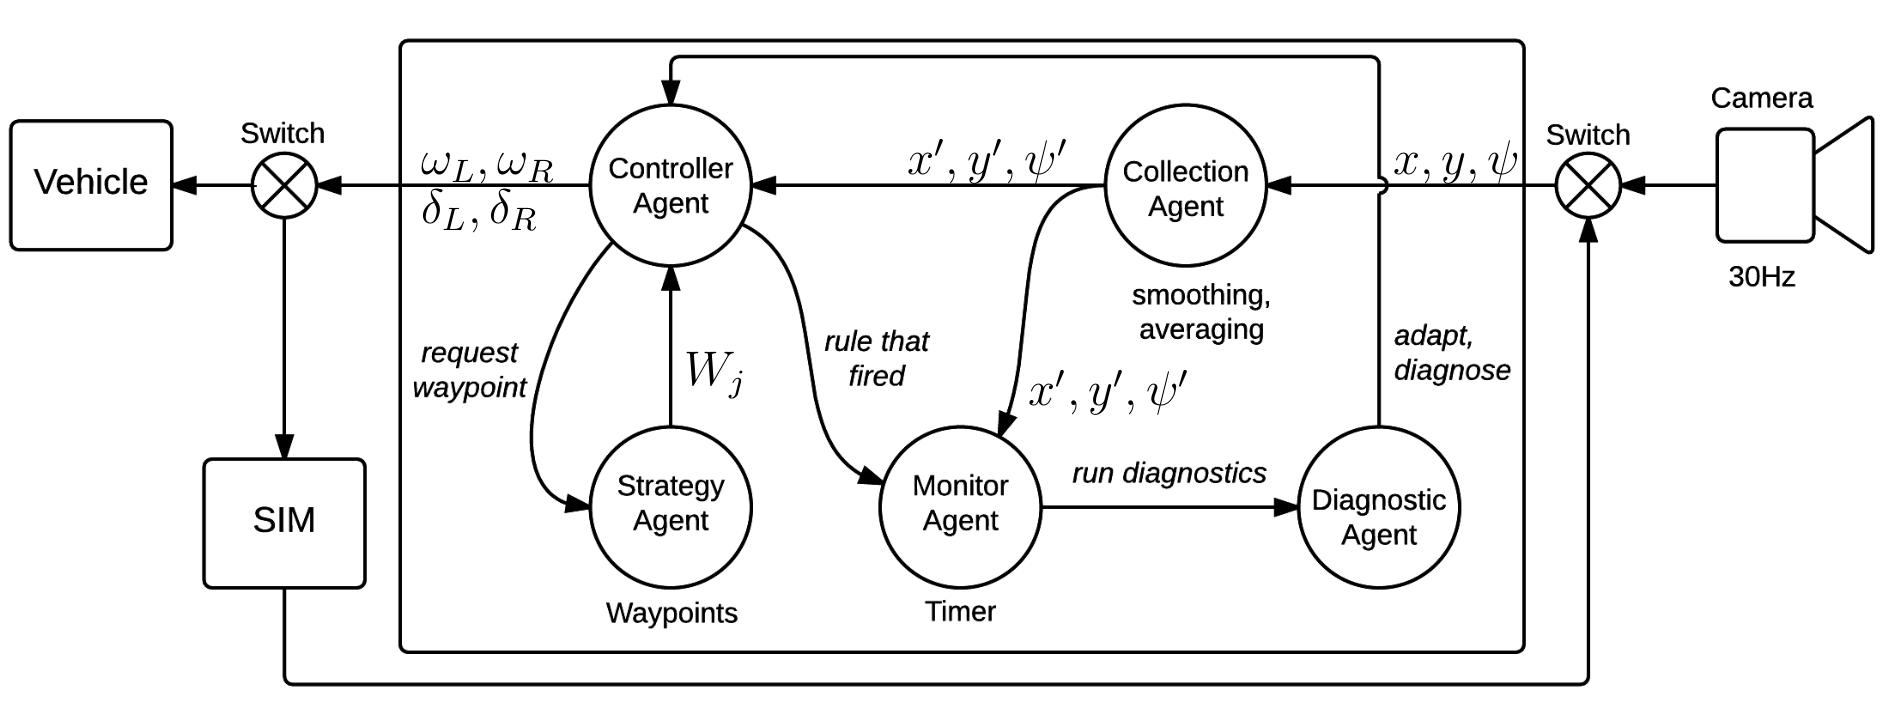
\includegraphics[width=\textwidth]{Files/Figures/mas_overview.png}
\caption[Diagram of Agent-based control architecture]{Diagram of Agent-based control architecture. Detailed information about each agent is provided in Section~\ref{subsec-agentDescription}. More info about the simulator (SIM) can be found in Section~\ref{sec-sim}. Note that the arrows between the agents do not reflect inter-agent messages---the communication is done by event processing, as described in Section~\ref{subsec-AgentScheduling}}
\label{fig_agents}
\end{figure*}

\subsubsection{Collection Agent}
\begin{description}
\item[\textbf{Precepts:}] \qquad $x, y, \psi$
\item[\textbf{Outputs:}] \qquad $x', y', \psi'$
\item[\textbf{Tasks:}] \qquad Collects high-speed data $x, y, \psi$ from either simulator or the camera, and computes smoothing and averaging of the data. Outputs estimated pose data $x', y', \psi'$ at a lower rate. There are several filtering options under consideration, e.g. an exponential moving average filter.
\end{description}

\subsubsection{Monitor Agent}
\begin{description}
\item[\textbf{Precepts:}] \qquad $x', y', \psi'$, active rule from rulebase
\item[\textbf{Outputs:}] \qquad issue diagnostics command
\item[\textbf{Tasks:}] \qquad Receives estimated position data from the collection agent, and movement being executed from the controller agent. Monitors performance of the vehicle, and in the case of unsatisfactory results, directs diagnostics agent to run diagnostics.
\end{description}

\subsubsection{Strategy Agent}
\begin{description}
\item[\textbf{Precepts:}] \qquad none
\item[\textbf{Outputs:}] \qquad $W_j$
\item[\textbf{Tasks:}] \qquad Stores list of waypoints. Sends next waypoint $W_j$ upon request.
\end{description}

\subsubsection{Controller Agent}
\begin{description}
\item[\textbf{Precepts:}] \qquad $x', y', \psi', W_j$
\item[\textbf{Outputs:}] \qquad $\delta_L, \delta_R, \omega_L, \omega_R$
\item[\textbf{Functions:}] \qquad Consists of one or more agents. Responsible for determining control inputs $\delta_L, \delta_R, \omega_L, \omega_R$ based on the vehicle pose $x', y', \psi'$ and the desired position $W_j$. When the vehicle reaches a waypoint, the agent requests new waypoint coordinates from the strategy agent. Runs maneuvers for diagnostics testing.
\end{description}

\subsubsection{Diagnostic Agent}
\begin{description}
\item[\textbf{Precepts:}] \qquad $x', y', \psi', W_j$
\item[\textbf{Outputs:}] \qquad computes likelihood of fault
\item[\textbf{Functions:}] \qquad Initiates diagnostics testing. Computes likelihood of failure. Determines if behavior must be adapted to compensate for faults.
\end{description}


\subsection{Agent Scheduling}
\label{subsec-AgentScheduling}
The scheduler is responsible for specifying when individual agents execute their assigned tasks. In this application scheduling is event-oriented rather than time oriented. Our scheduler is loosely based on the scheduler used in the RePast agent-based toolkit~\cite{REPAST}.

The scheduling process can be abstractly thought of as a sequence of hooks on a wall (see Fig \ref{fig:2}). An agent is "hung" on a hook if it is supposed to execute some task at some future time. However, time is relative, not absolute--i.e., hooks are not associated with some specific time nor does hook spacing reflect time intervals; hooks merely establish a partial ordering of agent tasks. For example, if agents $x, y,$ and $z$ are hung on hooks three, four and seven respectively, this simply says agent $x$ performs some task before agent $y$ which performs some task before agent $z$. Hooks therefore just order agent behaviors with respect to each other. Only one agent can be hung on a particular hook because agents do not execute tasks concurrently. We say an agent is \textit{stepped} if it is directed to perform some action or task.
 
The entire scheduling process is event driven. A first-in-first-out (FIFO) buffer is used as an event queue. As agents perform assigned tasks---i.e., they are stepped by the scheduler---they may post events in the FIFO, which might cause other agents to be stepped at a later time. Events have a header and a body. The header tells which agent posted the event, the event type and possibly a timestamp. The body contains attributes unique to the event. 

The scheduler unloads the buffer, analyzes the events, and processes events by stepping a specific agent. Events are pulled from the FIFO as quickly as possible, but stepping agent is deferred while the FIFO is not empty. All the scheduler does at this time is to decide upon which hook to hang the event. Some shuffling of agents already hung on hooks may occur depending on the priority of the event. When the FIFO is empty, the scheduler starts pulling agents off of hooks in a "first-hung-first-pulled" order and steps them. A stepped agent may be provided information from the body of the event that prompted it being stepped.

A simple example will help to clarify. Suppose the controller agent has just output new $\delta$ and $\omega$ values. This agent would post a ``new $\delta / \omega$ output'' event in the event queue. The body of this event would identify which rule in the rule base fired, so the commanded vehicle movement is recorded. When offloaded from the FIFO the scheduler would hang a monitor agent tag on a hook along with the rule ID extracted from the event body. Once the FIFO is empty, the scheduler pulls the monitor agent tag off of the hook and steps the monitor agent to commence observing the vehicle movement. The monitor agent would be informed at that time which rule fired.

\begin{figure}
\centering
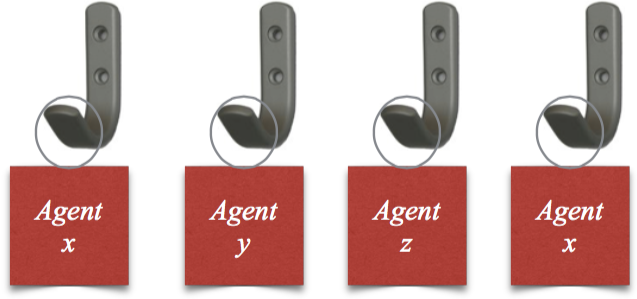
\includegraphics[width=0.75\textwidth]{Files/Figures/sch.png}
\caption[Agent scheduling example]{An example showing agents hanging on hooks waiting to be stepped by the scheduler. The left-to-right order reflects the relative ordering of the agent stepping.}
\label{fig:2}
\end{figure}


\section{Agent Implementation}
\label{sec-agentImplementation}
This section describes each of the agents mentioned above in more depth, including the implementation details.

\subsection{Controller Agent}
\label{subsec-controlerAgent}
This agent computes the $\delta$ and $\omega$ values needed to move the vehicle between waypoints. The vehicle will typically have to adjust its course as it moves along a trajectory. However, that does not mean new $\delta$ values are needed at the beginning of each wing beat.

There are four control inputs to the vehicle available (specifically $\delta_L, \delta_R, \omega_L, \omega_R$), but only two actuators (the left and right wing) thus the control inputs are not independent. This situation can be described as \textit{under-actuated} vehicle, which means we cannot control the position and course independently, and that creates a greater challenge for the controller agent. For example, if the vehicle is moving forward and is heading slightly left off the desired course, it can't turn right without affecting the forward motion. 

An arbitrary position and orientation can be achieved by a combination of linear motion (forward/backward movement) and rotation of the robot. Forward motion is done by increasing both $\delta_L$ and $\delta_R$ while rotation is achieved by increasing $\delta_L$ and decreasing $\delta_R$ and vice versa. Note that although backward movement is possible, it is not used in this case. Required movements are summarized in Table~\ref{tab-cmd}.

The vehicle is required to make two distinct turns -- a "hard" turn -- a rotation of $90\deg$ that is used for evasive maneuvers, and a "partial" turn, used for slight course corrections. Each turn requires different values of $\delta_L, \delta_R$, but the direction of change in $\delta$ is the same for both turns. The values of $\delta$ will be stored in a look-up table. Increasing $\omega_L$ or $\omega_R$ (while keeping the same relative value of $\delta$) creates stronger moments and forces, which might be necessary for faster movement, especially rotation. Suitable values for $\omega_L$ and  $\omega_R$ have yet to be determined.

The vehicle must make specific movements to follow a trajectory and a rule base determines which movements will be needed. These rules are organized in a  \textit{subsumption architecture}~\cite{brooks} (see Section~\ref{sec:subsumption_arch} for details).  Under this architecture, all control rules have an IF-THEN syntax. The rule base consists of the rules shown in Table~\ref{tab-subsum}. Each movement indicated in a rule's consequent has an associated set of $\delta$ and $\omega$ values, which are extracted via a table lookup.

A subsumption architecture consists of a series of layers where lower layer rules produce simple, critical behavior such as avoiding obstacles while higher levels produce more sophisticated behavior needed for trajectory following. Higher level behavior subsumes lower level behavior. A subsumption architecture is ideal for navigation control in dynamic physical environments. It permits reactive behavior without resorting to prior path planning because there is no world model required.

\begin{table}
\centering
\renewcommand{\arraystretch}{1.7}
\begin{tabular}{>{\small}l>{\small}c}
\hline
Movement & Control Input\\
\hline
\rowcolor{Gray}
Move Forward & $\delta_L \uparrow $ \& $ \delta_R \uparrow$ (identical)\\
Left Turn & $\delta_L  \downarrow $ \& $ \delta_R  \uparrow$ (opposite)\\
\rowcolor{Gray}
Right Turn & $\delta_L \uparrow $ \& $ \delta_R  \downarrow$ (opposite)\\
Idle & $\delta_L = \delta_R = 0$\\
\rowcolor{Gray}
Increase velocity & $\omega \uparrow$\\
Decrease velocity & $\omega \downarrow$\\
\hline
\end{tabular}
\newline
\caption[Required vehicle movements]{Required vehicle movements. $\uparrow, \downarrow$ indicate direction of change, not its magnitude.}
\label{tab-cmd}
\end{table}

Layer one has the highest priority. If the vehicle reaches the borders of the perimeter (in this case walls of the water tank), it will turn right to avoid the collision. The second highest priority detects whether the vehicle reached the desired waypoint $W_j$\footnote{The vehicle reaches waypoint $W_j$ if it is within distance $\epsilon$ of that waypoint.}. At that time, the controller agent acquires the coordinates of the next waypoint on the trajectory $W_{j+1}$ from the strategy agent.

A new waypoint should be requested promptly to prevent the vehicle from unnecessary course corrections and large control actions. The third layer ensures that if the vehicle is pointing at the waypoint, it will move towards the waypoint. If it is not pointing in the right direction, layers four and five will turn the vehicle until it is pointing right at the waypoint, so the third layer (i.e. ``move forward'') takes control. Finally, if there is nothing better to do, the vehicle idles at its current location until it gets new commands.

\begin{table}
\centering
\renewcommand{\arraystretch}{1.7}
\begin{tabular}{>{\small}c>{\small}l}
\hline
Layer & Behavior\\
\hline
\rowcolor{Gray}
6 & \textbf{if} true \textbf{then} \textit{Idle} \\
5 & \textbf{if} heading left \textbf{then} \textit{Partial right turn}\\
\rowcolor{Gray}
4 & \textbf{if} heading right \textbf{then} \textit{Partial left turn}\\
3 & \textbf{if} heading at waypoint \textbf{then} \textit{Move forward}\\
\rowcolor{Gray}
2 & \textbf{if} at waypoint $W_j$ \textbf{then} Get new waypoint $W_{j+1}$\\
1 & \textbf{if} outside perimeter \textbf{then} \textit{Hard right turn}\\
\hline
\end{tabular}
\newline
\caption[Controller agent subsumption architecture]{Scheme of Controller agent subsumption architecture, Layer 1 has the highest priority.}
\label{tab-subsum}
\end{table}

\subsection{Monitor Agent}
\label{subsec-monitorAgent}

This agent is responsible for monitoring the vehicle's performance. During normal vehicle operation, the controller agent posts an event every time a new $\delta$ and/or $\omega$ value is sent to the split-cycle oscillator. That event identifies the specific rule that fired, so the monitor agent knows the expected movement (e.g., \textit{hard right turn}) and, when stepped by the scheduler, begins tracking the movement. If the vehicle's movement doesn't match the expected movement, the monitor agent will post a ``poor performance'' event in the event queue. No event is posted if the behavior is okay. The scheduler will process this poor performance event by stepping the diagnostic agent to run diagnostics.


\subsection{Diagnostic Agent}
\label{subsec-DiagnosticAgent}
This agent assesses the vehicle's reliability. The vehicle has no specific fault detection and isolation capability. It is worth noting that under such circumstances there is, from a behavioral standpoint, no real difference between a vehicle mechanical failure or a sensor failure since both produce the same outcome---an inability to follow the desired trajectory. Nevertheless, rather simple diagnostic routines can identify degrading behavior even if the exact cause is not known.

Diagnostics could be performed at regular intervals. For example, every 5 minutes of flight time the vehicle could temporarily idle and then quickly run the diagnostics. However, a more practical approach is to exploit the online learning performed by the monitor agent. The monitor agent will trigger the diagnostics if and only if a degraded performance is observed.

Faults are detected using a Bayesian type of behavior monitor where \textit{likelihood functions} give a qualitative measure of maneuver capability. The idea behind diagnostics is simple: command the vehicle to perform some maneuver and see if it can do it within a prescribed time frame. A rotation through some angle---e.g. $\pi/2$ radians---is a simple and non-trivial maneuver since it requires $\delta_L \neq \delta_R$. The precise $\delta$ values are stored in a table as described previously. Note that a complete diagnostic would require the vehicle to rotate in both directions. Pose samples $\hat{\Psi}_n = (\hat{\psi}_1, \hat{\psi}_2, \ldots, \hat{\psi}_n )$ can be recorded by diagnostic agents over some time window and the associated sample mean and sample variance are easily computed. This information is sufficient to construct a Gaussian \textit{pose density function}:

\begin{equation}
f(\hat{\psi}) = \frac{1}{\sigma_\psi \sqrt{2\pi}}\exp \left( -\frac{(\hat{\psi} - \overline{\psi})^2}{2\sigma_\psi^2} \right)
\label{eq-like}
\end{equation}

\noindent where $\overline{\psi}$ is the sample mean and $\sigma^2_\psi$ is the sample variance.

The control agent outputs a specific $\delta_L$ and a $\delta_R$, which are expected to produce some change in pose. Thus, the control agent has some expected pose movement $E[\psi]$ in mind. A diagnostic agent uses the pose density function $f(\hat{\psi})$ to compute the likelihood of $E[\psi]$ given the pose data samples $\hat{\Psi}_n$. This concept is illustrated in Figure~\ref{fig_like}.

\begin{figure}
\centering
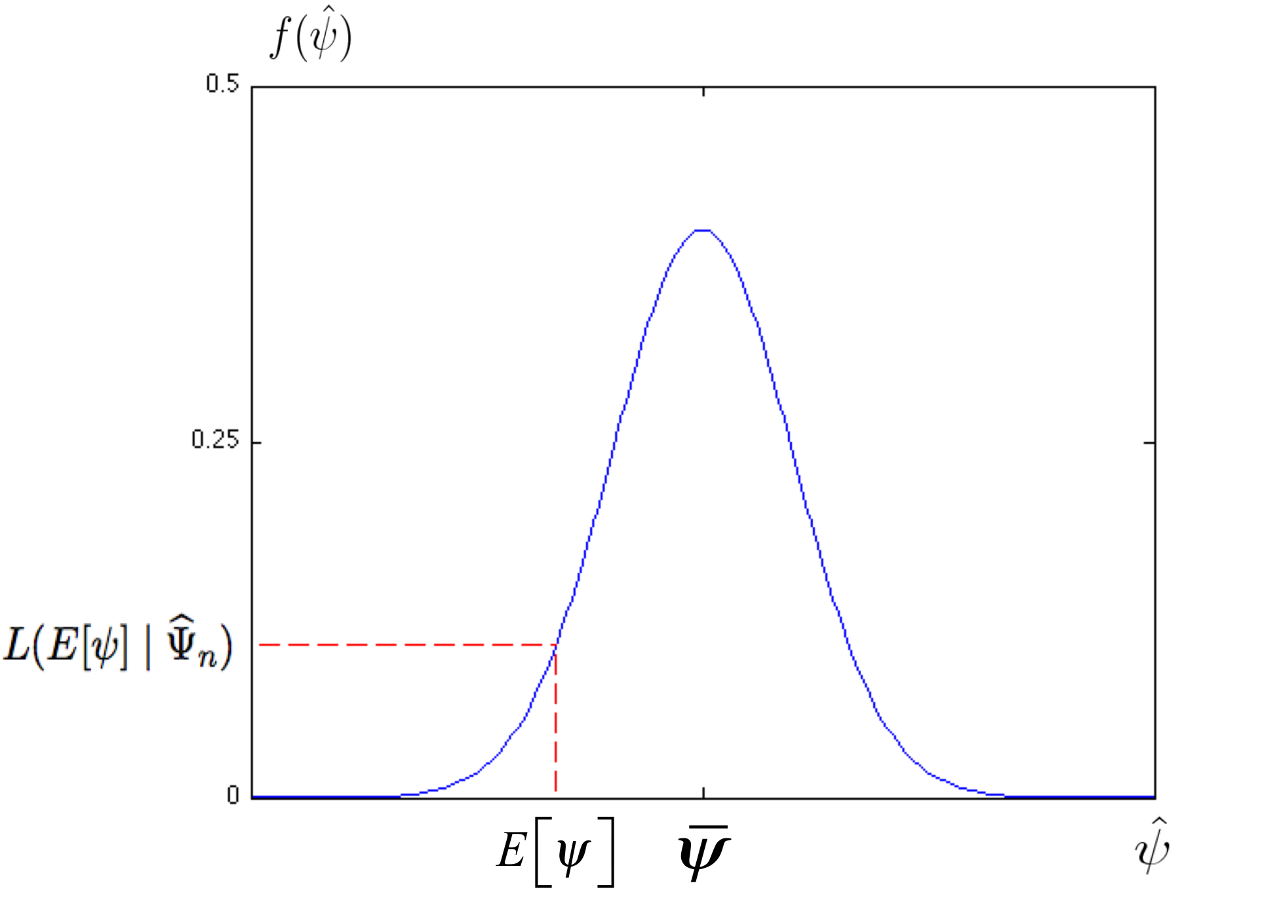
\includegraphics[width=0.8\textwidth]{Files/Figures/like.png}
\caption[Pose density function]{Calculation of likelihood of getting the expected pose from a pose density function
centered at the sample mean of the $n$ rotation estimate data samples $\hat{\Psi}_n$}
\label{fig_like}
\end{figure}
A high likelihood suggests the vehicle mechanical hardware and sensor hardware are normally operating while a low likelihood indicates something is wrong. Dividing the likelihood function value by the sample mean (or equivalently just ignoring the $1/(\sigma_\psi \sqrt{2\pi})$ coefficient in Eq.~\ref{eq-like}) makes $L ( E[\psi]|\hat{\Psi}) \in [0, 1]$. Then 'high' and 'low' likelihoods are defined by a threshold parameter $\lambda$ on the unit interval. That is, $L (\cdot) < \lambda$ indicates a low likelihood the vehicle can maneuver properly, and some corrective action is required. The only possible recovery mechanism is to adapt the vehicle's behavior by modifying the rules in the rule base. The next section describes how this adaption is done.


\section{Agent Online Learning}
\label{sec-AgentAdaptation}
There are two times when online learning is required. Learning is used to identify appropriate  $\delta$ and $\omega$ values needed for control of the vehicle. This section discusses the details of the learning process.

\subsection{Initial Learning}
\label{subsec-FirstStageAdaptation}
Every vehicle is slightly different due to inherent non-linearities such as slip between linkages and manufacturing imperfections. Thus, the same $\delta$ and $\omega$ values cannot be used for every vehicle; they must be learned. First the vehicle learns values needed to execute the basic movements in Table~\ref{tab-cmd}. These values are then linked to rule consequents from Table~\ref{tab-subsum}. The $\delta$ and $\omega$ values will be determined during this initial learning phase using a combination of extrinsic and intrinsic evolution.
The needed parameters will be evolved using a (1,10)-ES. The genotype is 

\[\left\{ {{\delta _L},{\delta _R},{\omega _L},{\omega _R}\ ;\ {\sigma _1},{\sigma _2},{\sigma _3},{\sigma _4}} \right\}\]

\noindent where the first 4 parameters are object parameters and the second 4 parameters, are strategy parameters used to control the mutation step size. The object parameters are mutated independently using a normal distribution and the appropriate strategy parameter. The equation for production of a new individual $y$ from a single parent $x$ is given as:

\begin{equation}
\delta_{L_y} = \delta_{L_x} + N(0,\sigma_{\delta_L})
\label{eq-1}
\end{equation}

where $N(0,\sigma_{\delta_L})$ is a normally distributed random variable with zero mean and a standard deviation of $\sigma_{\delta_L}$. The other \textit{object parameters} with their respective \textit{strategy parameters} are mutated the same way as described in the Equation~\ref{eq-1}. Most likely a linear reduction schedule will be sufficient for adapting the strategy parameters.  

The vehicle will be placed in its operational environment -- i.e. a water tank -- and object parameter values will be intrinsically evolved for each movement. The initial object parameter values will be evolved extrinsically using an in-house developed simulator. %Intrinsic evolution will be run with onboard computing resources.

The monitor agent observes the behavior of each evolved object parameter set and terminates the evolutionary algorithm for a particular rule when acceptable behavior is achieved. The goal here is not to achieve optimal movements but rather smooth and repeatable correct movements. Thus, fitness will be computed from the average behavior over a small number of trials. After learning is completed, the evolved values will be stored in a library (i.e. a look-up table). Once all rules are evolved the vehicle is ready for trajectory following.

\subsection{In-Flight Learning}
\label{subsec-SecondStageAdaptation}
Rules learned during the initial learning phase perform well during normal flight, but in the presence of faults, it will be necessary to adapt them. This online learning phase is performed continuously. Each time a rule fires the monitor agent is informed, so it knows what maneuver was commanded. The monitor agent observes the $x', y,' \psi'$ pose parameters and determines if the performance is within limits or is degrading. Thus, the monitor agent continuously learns about how the vehicle is performing. If the observed behavior deviates too much from the expected behavior, then diagnostics are run. If the diagnostics confirm the behavior has degraded below some threshold, then the rule base is adapted. Adaption, described below, entails modifying rules’ consequents to restore vehicle’s functionality.

\subsection{Rule-base Adaptation}
\label{subsec-FaultDetection}
Given the size and weight restrictions, which don’t allow us to use conventional fault recovery methods such as redundant hardware, it is not possible to recover from every possible fault. We, therefore, restrict the adaption to cover only a small subset of predefined faults. The recovery mechanism relies on adapting new consequents for rules from Table~\ref{tab-subsum} so that the desired motion (i.e. \textit{Partial left turn}) is still achievable. These new $\delta$ and $\omega$ values will be intrinsically evolved just like the initial online learning was done. The question is how do we intrinsically evolve new parameters for specific faults?

We will borrow concepts used in conventional \textit{failure modes \& effects testing} (FMET). In this type of testing, a set of predefined faults is inserted into the system under test one at a time, and their effect is observed. This testing is always conducted in a laboratory environment where the effects are closely monitored and controlled to prevent damage to the system. In this particular research effort, "faults" such as using different wing sizes or a stuck linkage will be intentionally put into the vehicle, and an evolutionary algorithm will then evolve new parameter values. As before, this evolutionary algorithm will run using onboard hardware resources. The evolved values will be added to the rule base library.

Under normal operation, a single set of $\delta_L, \delta_R, \omega_L$ and $\omega_R$ values is sufficient to perform the maneuvers shown in Table~\ref{tab-cmd}. However, under faults most likely a sequence of $\delta$ and $\omega$ values will be required, with a new set generated every few hundred wingbeats (because of the slow vehicle dynamics). This sequence of values can be intrinsically evolved too. In this case, the genotype described earlier must be expanded to handle multiple $\delta$ and $\omega$ values for each maneuver.

Of course prior to initiating fault recovery operations \textit{fault detection \& isolation} (FDI) must be done. This process detects if a fault exists and tries to isolate it to a specific subsystem or component. Since the ability to recover from faults on the vehicle is severely limited, isolation is unnecessary. Fortunately, detection is rather straightforward. As stated above, the monitor agent is continuously learning about the vehicle capabilities; it can, therefore, detect poor performance by comparing observed behavior against expected behavior. If the behavior is poor, it will post an event in the event queue. The scheduler would then step the diagnostic agent to start diagnostics. Diagnostics should be able to confirm both degraded performances and identify which of the pre-defined faults is present. The abstract sequence of commands used during FDI is summarized in Algorithm~\ref{algo:fdi}.

\begin{algorithm}
\caption{The abstract sequence of commands used during FDI}
\label{algo:fdi}
\begin{algorithmic}
\STATE 1. Monitor Agent (MA) detects unsatisfactory performance and posts an event in event queue;
\STATE 2. Diagnostics Agent (DA) is scheduled to perform diagnostics;
\STATE 3. DA posts a diagnostic event.  Controller Agent (CA) stops waypoint following and enters diagnostics mode;
\STATE 4. CA starts the test maneuver;
\STATE 5. MA monitors test progress and passes results to DA;
\STATE 6. DA computes the likelihood of a fault;
\STATE 7. If DA detects no problem, it posts a regular operation event. CA resumes waypoint following;
\STATE 8. If DA detects a problem, it posts a faulty operation event. CA extracts new rule base from the library;
\end{algorithmic}
\end{algorithm}

Essentially we will build a library of rules for both the fault-free and the faulty vehicle.  Once FDI is finished fault recovery begins. Recovery only requires replacing the current controller agent's rule base with the appropriate pre-stored rule base associated with the identified fault from the library. Thus, fault recovery can be done very quickly. 

In this chapter we presented the MAS and explained how we use it to solve the problem of autonomous waypoint following and fault recovery. In next chapter we will describe the experimental results of our work.
